\documentclass[tikz,border=1.2mm]{standalone}
\usetikzlibrary{decorations.pathmorphing}

\begin{document}
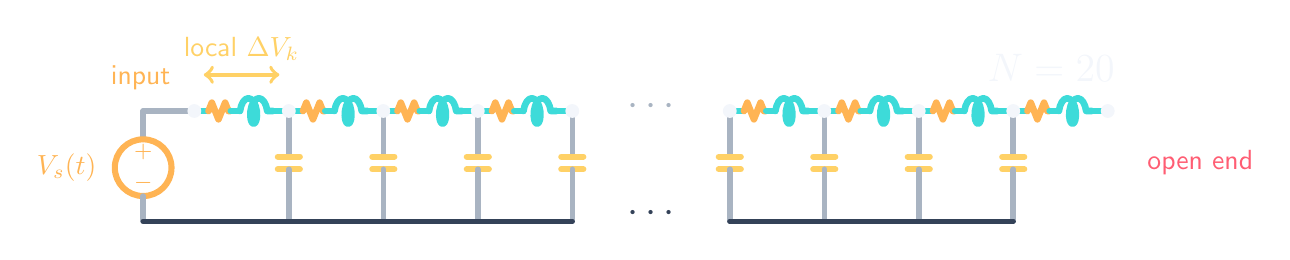
\begin{tikzpicture}[
    x=1cm,
    y=1cm,
    line cap=round,
    line join=round,
    every node/.style={font=\sffamily},
]
\definecolor{psText}{HTML}{F3F6FB}
\definecolor{psMuted}{HTML}{A9B4C2}
\definecolor{psStroke}{HTML}{344258}
\definecolor{psCyan}{HTML}{3DDBD9}
\definecolor{psOrange}{HTML}{FFB454}
\definecolor{psRed}{HTML}{FF5D73}
\definecolor{psYellow}{HTML}{FFD166}

\tikzset{
    wire/.style={draw=psMuted,line width=2.0pt},
    topwire/.style={draw=psCyan,line width=2.2pt},
    bus/.style={draw=psStroke,line width=1.9pt},
    resistor/.style={draw=psOrange,line width=2.4pt,decorate,decoration={zigzag,amplitude=3.0pt,segment length=4.8pt}},
    inductor/.style={draw=psCyan,line width=2.4pt,decorate,decoration={coil,aspect=0.45,segment length=3.8pt,amplitude=4.6pt}},
    capplate/.style={draw=psYellow,line width=2.2pt},
    sourcecircle/.style={draw=psOrange,line width=2.2pt},
}

\newcommand{\sectioncell}[2]{
    \draw[topwire] (#1,0) -- ({#1 + 0.18},0);
    \draw[resistor] ({#1 + 0.18},0) -- ({#1 + 0.46},0);
    \draw[topwire] ({#1 + 0.46},0) -- ({#1 + 0.58},0);
    \draw[inductor] ({#1 + 0.58},0) -- ({#2 - 0.20},0);
    \draw[topwire] ({#2 - 0.20},0) -- (#2,0);
}

\newcommand{\shuntcap}[1]{
    \draw[wire] (#1,0) -- (#1,-0.58);
    \draw[capplate] ({#1 - 0.14},-0.58) -- ({#1 + 0.14},-0.58);
    \draw[capplate] ({#1 - 0.14},-0.74) -- ({#1 + 0.14},-0.74);
    \draw[wire] (#1,-0.74) -- (#1,-1.40);
}

\sectioncell{-5.70}{-4.50}
\sectioncell{-4.50}{-3.30}
\sectioncell{-3.30}{-2.10}
\sectioncell{-2.10}{-0.90}

\sectioncell{1.10}{2.30}
\sectioncell{2.30}{3.50}
\sectioncell{3.50}{4.70}
\sectioncell{4.70}{5.90}

\draw[wire] (-6.35,0.00) -- (-5.70,0.00);
\draw[wire] (-6.35,0.00) -- (-6.35,-0.36);
\draw[sourcecircle] (-6.35,-0.72) circle (0.36);
\node[text=psOrange] at (-6.35,-0.52) {\footnotesize $+$};
\node[text=psOrange] at (-6.35,-0.92) {\footnotesize $-$};
\node[text=psOrange,anchor=east] at (-6.82,-0.72) {$V_s(t)$};
\draw[wire] (-6.35,-1.08) -- (-6.35,-1.40);

\foreach \x in {-4.50,-3.30,-2.10,-0.90,1.10,2.30,3.50,4.70} {
    \shuntcap{\x}
}

\draw[bus] (-6.35,-1.40) -- (-0.90,-1.40);
\draw[bus] (1.10,-1.40) -- (4.70,-1.40);

\foreach \x in {-5.70,-4.50,-3.30,-2.10,-0.90,1.10,2.30,3.50,4.70,5.90} {
    \fill[psText] (\x,0) circle (2.5pt);
}

\node[text=psMuted] at (0.10,0.05) {\Large $\cdots$};
\node[text=psStroke] at (0.10,-1.30) {\Large $\cdots$};
\node[text=psOrange,anchor=east] at (-5.88,0.42) {input};
\node[text=psRed,anchor=west] at (6.28,-0.65) {open end};
\node[text=psText,anchor=west] at (4.25,0.55) {\Large $N = 20$};

\draw[<->,draw=psYellow,line width=1.35pt] (-5.58,0.46) -- (-4.62,0.46);
\node[text=psYellow,anchor=south] at (-5.10,0.52) {local $\Delta V_k$};
\end{tikzpicture}
\end{document}
